% Chapter 2
\chapter{Conclusions and Future Work} % Main chapter title
\label{Chapter6} % For referencing the chapter elsewhere, use \ref{Chapter2} 
\minitoc
%----------------------------------------------------------------------------------------

%% Define some commands to keep the formatting separated from the content 
%\newcommand{\keyword}[1]{\textbf{#1}}
%\newcommand{\tabhead}[1]{\textbf{#1}}
%\newcommand{\code}[1]{\texttt{#1}}
%\newcommand{\file}[1]{\texttt{\bfseries#1}}
%\newcommand{\option}[1]{\texttt{\itshape#1}}

%----------------------------------------------------------------------------------------

The presented master thesis draws two types of conclusions, one related to the actual performance of the building and one related to the data mining techniques. Lastly in this chapter, propositions for future work take into consideration the feedback from Synergy BTC AG's specialists.

\section{Conclusions}
\subsection{Building performance} 


The proposed learning models and the correspondent visualizations contributed to the gain of information about the interactions between occupants and the studied building. The proposed approach aims to be applicable for other multivariate building datasets as well. For our studied building, we can conclude for each of the proposed model, the following:\\


The proposed \textit{GaHMM profile} model is effective to discover the daily profiles of the studied building dataset. The best trained models allows to perform the time-depending clustering of similar daily profiles. In average, from 25 to 40 cluster profiles were needed to summarize the information of the three years of time series for each variable in the dataset. Therefore more than 1200 daily profiles can be found for the whole dataset. For each particular variable of the dataset, each cluster profile was well defined by the mean vector and the corresponding standard deviation for each hour. This level of detail, in combination with the hierarchical agglomerative clustering represent a powerful tool for discovering the motif and discord cluster profiles of any variable of interest. The interviewed experts only needed a quick glance to the dendrogram to differentiate the motif and discord profiles of a selected variable. They agreed that the presented approach provides a direct feedback about the gap that exists between the desired performance and the actual performance of a building.   \\ 

The proposed \textit{GaHMM seasonal} model is an innovative aid to understand how seasons affect the daily profiles of a building. Changes of patterns of daily profiles in buildings are inevitable when seasons change across the years. The seasonal labels obtained from \textit{GaHMM seasonal} model assists the filtering process according to the interest of the researcher. Using the seasonal labels in conjunction with the \textit{GaHMM profile} model helped us to discover the way patterns change across seasons and years. Furthermore, using the seasonal label we observed that is possible, for instance, to identify motif and discord profiles for a selected season.  \\

The proposed \textit{GaHMM interactional} model was a robust model able to explain the typical correlations between variables in the studied multivariate dataset. This model helped to understand how a set of variables keep on a negative linear correlation with the $CO_2$ levels, when OcP is likely to occur ( assuming that $CO_2$ levels were produced by the occupants). Furthermore, irregular situations could be spotted in periods where the negative correlation between variables does not match with the typical $CO_2$ profiles. These situations could be associated to sensor faults, irregular position of the sun blinds, irregular temperatures among others issues. Unfortunately, there is no ground truth for approving this hypothesis. Nevertheless, we believe that the \textit{GaHMM interactional} model could assist in the detection of OcP.   \\ 

The potential of all the GaHMM models was tested in a case study presented in section \ref{section:case_study_1} where the North-East and South-West ventilation system were compared. The label data frame assisted in the filtering process and a discovered period maintenance of the building was found by using the labels produced by \textit{GaHMM interactional} model. Anomalous daily profiles were found in the North ventilation system before and during the maintenance period. After the maintenance period, there were no new occurrences of anomalous daily profiles. It was hence also proved that after the maintenance period, the patterns of the daily profiles were modified in significant ways for the $CO_2$ level variable. 

\subsection{Data mining techniques}

Using a Big-Data base approach proved to be a helpful mechanism for retrieving information from several collections in different formats/structures. This was particularly advantageous during the running of the proposed algorithm, and in the saving and visualization of partial results but also throughout the entire knowledge discovery process.    \\


By comparing SAX and GaHMM-profile model, we observed that our proposition is more precise in forming the cluster profiles of the variables. This was seen in the evaluation of the clustering quality where we observed that each of the daily profiles fits very well in the shape of the correspondent clustering profile. This is beneficial at the time of doing the discrimination between motif and discord cluster profiles. The use of the hierarchical dendrogram facilitates the definition of the manual threshold that discriminates both motif and discord profiles. We believe that this technique is very powerful and that its use could be extended to another domains.   

Following to our experiences during this project, we have realized that due to the complexity of the multivariate dataset, developing information visualization mechanisms that communicate the internal dynamics of the building is a very hard task. However, we also observed that our approach is a powerful tool to summarize information of a time series. The discovered cluster profiles can be used for different purposes, and they could serve to implement new and meaningfully mechanisms for visualizing the dynamics of a building. The use of the label data frame could be a good ally in representing information about a building, since they summarize the fluctuation of the variables in cluster labels, thus the researcher can filter the information according his interests and needs. We believe that our proposed approach can be useful for powerful visualizations that assist the stakeholders get an effective grasp of the internal dynamics of a building.   



\section{Future work}
\label{future}

Regarding knowledge discovery about building dynamics, our approach can be useful concerning information visualization systems helping to increase the knowledge of the actual performance of the building. New data visualizations can be proposed by using the label data frame exposed in section \ref{section:case_study_1}. For example, we propose in figure \ref{fig:future_work}, a possible visualization where the stakeholders can navigate and find the discord profiles of interest. A discord profile can be selected by doing a click over the small fault squares; the user can then compare the discord profile against the expected profile of that day. The expected profile area can be calculated by applying our proposition that was explained in section \ref{sec:pract_app}.      


\begin{figure}[h!]
  \vspace{0.5em} %better style
  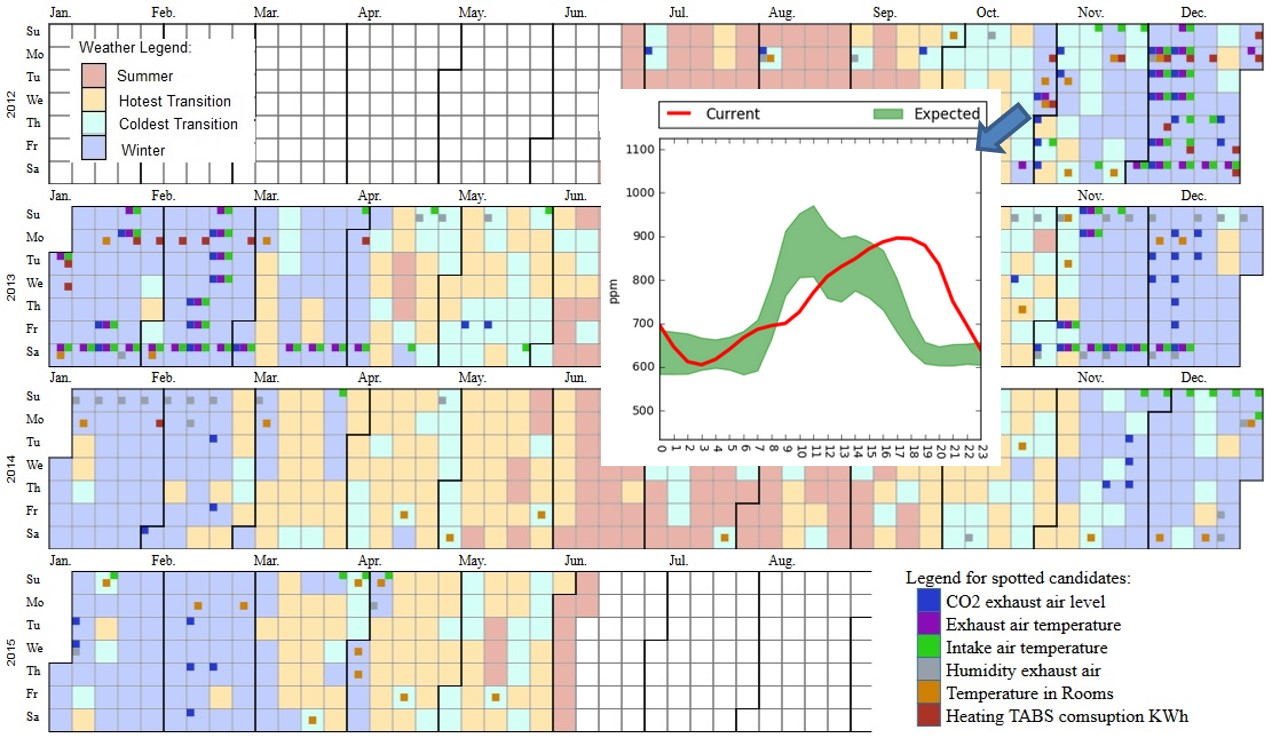
\includegraphics[scale=0.4]{Figures/future.jpg}
  \caption{Possible interactive visualization}
  \label{fig:future_work}
\end{figure} 

We consider that the feedback coming from the building expert in section \ref{comments} are important for future work in this domain, we summarize these points here:   

\begin{itemize}

\item A practical application of fault detection can be implemented and evaluated (section \ref{sec:pract_app}). Experts propose our approach, that is, \textit{GaHMM profile} and HAC approach for this purpose. Using the ground truth of the dataset, the evaluation can be done by using indicators such as the false positives and false negative rates, and a metric indicator for reliability. 

\item An evaluation of cost/benefits must be done. The question to solve is: How much it is going to cost to achieve a 'perfect' performance of the building (i.e. going from discord profiles to motif profiles)?. 

\item Apply our approach in critical variables (i.e. variables used in controller devices) can be a motivation for further studies. 

\item Is there a way to use our approach to discover the best moment to sell energy to the grid?

\item If the user awareness increases concerning the dynamics of building, people would be empowered to demand comfort enhancement, lower energy consumption or any other aspect of interest to the user. Can our approach assist the user in this purpose?

\end{itemize}
    


 







